\documentclass[14pt,a4paper]{extarticle}

\usepackage{fontspec}
\setmainfont{Times New Roman}[Ligatures=TeX]
\setmonofont{Courier New}
\newfontfamily\cyrillicfonttt{Courier New}

\usepackage{polyglossia}
\setmainlanguage[forceheadingpunctuation=false]{russian}
\setotherlanguage{english}

\usepackage{geometry}
\geometry{left=30mm,right=15mm,top=20mm,bottom=20mm}

\usepackage{setspace}
\onehalfspacing
\usepackage{indentfirst}

\usepackage{graphicx}
\usepackage{array}
\usepackage{float}
\graphicspath{{figures/}}
\usepackage{caption}
\captionsetup{font=normalsize,skip=8pt,justification=centering}
\renewcommand{\labelitemi}{\textbullet}

\usepackage{pdfpages}
\usepackage{hyperref}
\hypersetup{hidelinks,unicode,pdftitle={Проектирование информационной системы валидации юридического лица для получения кредита}}

\setlength{\parskip}{0pt}
\clubpenalty=10000
\widowpenalty=10000
\emergencystretch=3em

\begin{document}

\IfFileExists{first_page.pdf}{%
\includepdf[pages=1,pagecommand={\thispagestyle{empty}}]{first_page.pdf}%
}{%
\begin{titlepage}
\thispagestyle{empty}
\centering
\setlength{\parindent}{0pt}
МИНИСТЕРСТВО НАУКИ И ВЫСШЕГО ОБРАЗОВАНИЯ РОССИЙСКОЙ\\
ФЕДЕРАЦИИ\\
ФЕДЕРАЛЬНОЕ ГОСУДАРСТВЕННОЕ АВТОНОМНОЕ\\
ОБРАЗОВАТЕЛЬНОЕ УЧРЕЖДЕНИЕ ВЫСШЕГО ОБРАЗОВАНИЯ\\
НАЦИОНАЛЬНЫЙ ИССЛЕДОВАТЕЛЬСКИЙ ЯДЕРНЫЙ УНИВЕРСИТЕТ\\
«МИФИ»\par
\vspace{28.3pt}
Институт интеллектуальных кибернетических систем\\
Кафедра кибернетики (№22)\\
Направление подготовки 09.04.04 Программная инженерия\par
\vspace{85pt}
{\bfseries Курсовая работа по моделированию предметных сред\\
и проектированию баз данных}\par
\vspace{28.3pt}
{\bfseries «Проектирование информационной системы\\
валидации юридического лица\\
для получения кредита»}\par
\vfill
\raggedright
\hfill
\begin{minipage}{0.62\textwidth}
Выполнил студент группы М26-514\\
Гришанов~Н.\,В.\\[0.9em]
Преподаватель\\
Тихомирова~Д.\,В.
\end{minipage}\par
\vspace{1.6em}
\centering
Москва 2026\par
\end{titlepage}
}

\renewcommand{\contentsname}{Содержание}
\tableofcontents
\newpage

\section{Обзор системы}

\subsection{Формулировка задания}

Необходимо спроектировать информационную систему валидации юридического лица для получения кредита. Система проверяет организацию по законодательству Российской Федерации и по кредитным условиям банка и завершает работу заключением. Заключение передаётся контуру выдачи. Договор, график платежей и зачисление остаются за границей системы. Период охлаждения потребительского кредита к проверке юридического лица не относится.

Организация подаёт заявку с суммой, сроком, валютой и целью. Вместе с заявкой учитываются люди, которые в ней участвуют, цепочка владения между юридическими лицами, обязательные проверки и показатели, сопоставленные с условиями продукта. Вывод по показателю~--- усиливает, ослабляет или блокирует~--- хранится в связи <<Учтено>> вместе с применённым весом и порогом. Обязательная проверка фиксирует соответствие норме. Срок хранения зависит от категории сведений: клиент, показатель, пакет заявки и кредитные условия живут отдельно.

\subsection{Назначение и цели создания системы}

Назначение~--- проверять юридическое лицо для получения кредита по одним правилам в офисе и в дистанционном канале. Карточка организации, согласия, проверки, показатели и условия общие для менеджера и автоматической проверки.

Цели:

\begin{itemize}
\item учёт организации, участия людей и владения между организациями;
\item фиксация согласия лица и организации на обработку сведений и на запрос кредитной истории;
\item обязательные проверки по норме с источником и датой;
\item учёт показателей в заявке: вес, порог и вывод по условиям этой заявки;
\item заявка на одних кредитных условиях, с корпоративным одобрением и обеспечением, когда сделка этого требует;
\item заключение с результатом, уровнем риска, сроком действия и причиной отказа;
\item четыре категории хранения: клиент, показатель, пакет и условия.
\end{itemize}

\subsection{Основные функциональные возможности системы}

\begin{itemize}
\item \textbf{Учёт юридического лица.} Наименование и организационно-правовая форма, ИНН, ОГРН и ОКВЭД, статус, адрес, лицензия. Статус и лицензируемый вид деятельности читаются из карточки организации.
\item \textbf{Учёт физического лица и участия.} ФИО, паспорт и дата рождения, гражданство и адрес. Участие хранит долю, вид связи и основание. Виды связи: учредитель, руководитель, бенефициар, представитель. Бенефициарный владелец~--- физическое лицо с долей более двадцати пяти процентов либо с возможностью контролировать организацию. Если такое лицо не установлено, для идентификации берётся единоличный исполнительный орган.
\item \textbf{Владение.} Связь двух юридических лиц: доля и основание. Одна сторона~--- владелец, другая~--- объект владения. Косвенная доля считается произведением долей по цепочке. Человек владеет шестьюдесятью процентами организации, а та~--- сорока процентами другой: косвенная доля во второй организации составляет двадцать четыре процента. Порог бенефициарного владения~--- более двадцати пяти процентов либо контроль, и во второй организации он не пройден. В первой организации этот человек~--- бенефициарный владелец. Промежуточная организация остаётся стороной владения.
\item \textbf{Согласие.} Цель обработки, основание и срок действия. Согласие даёт физическое лицо или юридическое лицо. Проверка ссылается на согласие, когда использует персональные данные или кредитную историю. Срок действия согласия хранится в самом согласии и срок хранения записи не заменяет.
\item \textbf{Обязательная проверка.} Вид и норма, результат, источник и дата. Проверка принадлежит заявке. Связь <<по лицу>> необязательна и нужна для полномочий, бенефициара и публичного должностного лица. Результат~--- пройдена или не пройдена. Непройденная проверка закрывает путь к положительному заключению. Вес у правовой проверки отсутствует: норма либо соблюдена, либо нет.
\item \textbf{Финансовая отчётность и показатель.} Организация ведёт отчёты: форма, период, валюта, дата составления. Отчёт содержит показатели. Показатель хранит вид и период, значение, источник и дату и может быть записан без отчёта, если источник~--- суд, налог или бюро. В заявку показатель попадает через связь <<Учтено>>: вес, порог и вывод. Вывод относится к этой заявке и этим условиям. Новая редакция условий оставляет уже записанный вес прежним.
\item \textbf{Заявка и кредитные условия.} Номер, дата и канал, сумма, срок и валюта, статус и цель проверки. Каналы: интернет-банк, офис, менеджер. Цели: первичное рассмотрение, увеличение лимита, пролонгация, замена обеспечения. Заявка ссылается ровно на одни кредитные условия: продукт и валюта, лимиты и срок, требование обеспечения. Новая редакция лимитов~--- новая запись условий. Повторная проверка~--- новая заявка.
\item \textbf{Корпоративное одобрение.} Орган и дата решения, вид сделки, одобренная сумма. Вид сделки~--- крупная сделка или сделка с заинтересованностью. Одобрение есть не у каждой заявки.
\item \textbf{Обеспечение.} Вид и предмет залога, оценка стоимости, действующее обременение. Заявка предлагает ноль или несколько обеспечений, когда условия продукта этого требуют.
\item \textbf{Заключение.} Результат проверки, уровень риска, срок действия, причина отказа. У заявки ноль или более заключений. Результат: положительный, положительный с ограничениями, отказ. Риск: низкий, средний, высокий, критический. Пересмотр добавляет новое заключение и сохраняет предыдущее. Связь заключения с показателем проходит через заявку и через <<Учтено>>.
\item \textbf{Правило хранения.} Категория сведений, основание и срок, событие начала отсчёта. Категория <<клиент>> покрывает физическое и юридическое лицо; участие и владение хранятся вместе с ними. Категория <<показатель>> покрывает показатель и финансовую отчётность. Категория <<пакет>> покрывает заявку, проверку, связь <<учтено>>, корпоративное одобрение, обеспечение и заключение. Категория <<условия>> покрывает редакции кредитных условий.
\end{itemize}

\subsection{Конкретизация предметной области (границы автоматизации)}

Предметная область~--- проверка организации до заключения по заявке на заданных условиях. В границе автоматизации остаются организация, люди и их участие, владение, согласия, заявки, обязательные проверки, отчётность и показатели, корпоративное одобрение, обеспечение и заключение. Договор, график платежей и зачисление остаются в контуре выдачи и в систему не входят.

\begin{itemize}
\item \textbf{Физическое лицо.} ФИО, паспорт и дата рождения, гражданство и адрес. Связь <<участвует>>: у участия ровно одно лицо, у лица~--- ноль или много участий.
\item \textbf{Участие.} Доля, вид связи, основание. Связь <<в организации>>: участие принадлежит ровно одной организации, у организации~--- ноль или много участий. Участие без организации не создаётся.
\item \textbf{Юридическое лицо.} Наименование и организационно-правовая форма, ИНН, ОГРН и ОКВЭД, статус, адрес, лицензия. Подаёт нуль или более заявок; у заявки организация ровно одна.
\item \textbf{Владение.} Доля и основание. Связь <<владеет>> указывает организацию-владельца: у записи владения владелец ровно один. Связь <<объект>> указывает организацию, которой владеют: объект тоже ровно один. Одна организация выступает владельцем и объектом в разных записях, и из таких записей собирается цепочка.
\item \textbf{Согласие.} Красная контрольная сущность: цель обработки, основание, срок действия. Его даёт физическое лицо либо юридическое лицо. По связи <<даёт>> у согласия ровно один давший, у лица и у организации~--- ноль или много согласий.
\item \textbf{Обязательная проверка.} Вид и норма, результат проверки, источник и дата. Связь <<проходит>>: проверка принадлежит ровно одной заявке, у заявки одна или несколько проверок. Связь <<допускает>>: у проверки не более одного согласия. Связь <<по лицу>>: у проверки не более одного участия.
\item \textbf{Финансовая отчётность.} Форма и период, валюта отчёта, дата составления. Связь <<ведёт>>: отчёт принадлежит ровно одной организации. Связь <<содержит>>: у показателя не более одного отчёта, у отчёта~--- ноль или много показателей.
\item \textbf{Показатель.} Вид и период, значение показателя, источник и дата. Связь <<входит>>: у записи <<Учтено>> ровно один показатель. Связь <<в заявке>>: у этой записи ровно одна заявка, у заявки~--- ноль или много учтённых показателей. Вес, порог и вывод стоят на ромбе <<Учтено>>.
\item \textbf{Заявка.} Номер, дата и канал, сумма, срок и валюта, статус и цель проверки. Связь <<на условиях>>: у заявки ровно одни кредитные условия, у условий~--- ноль или много заявок.
\item \textbf{Кредитные условия.} Продукт и валюта, лимиты и срок, требование обеспечения. Общая рамка для заявок разных организаций. Срок жизни редакции задаёт категория хранения <<условия>>.
\item \textbf{Корпоративное одобрение.} Орган и дата решения, вид сделки, одобренная сумма. Связь <<одобрена>>: у одобрения ровно одна заявка, у заявки~--- ноль или много одобрений.
\item \textbf{Обеспечение.} Вид и предмет залога, оценка стоимости, действующее обременение. Связь <<предлагает>>: у обеспечения ровно одна заявка, у заявки~--- ноль или много предметов.
\item \textbf{Заключение.} Результат проверки, уровень риска, срок действия, причина отказа. Связь <<рассматривается>>: у заключения ровно одна заявка, у заявки~--- ноль или много заключений. Заключение существует только вместе с заявкой и действует до указанной даты.
\item \textbf{Правило хранения.} Контрольная сущность: категория сведений, основание и срок, событие начала отсчёта. Категория <<клиент>> покрывает лицо, организацию, участие и владение; категория <<показатель>>~--- показатель и отчётность; категория <<пакет>>~--- заявку, проверку, <<учтено>>, одобрение, обеспечение и заключение; категория <<условия>>~--- кредитные условия.
\end{itemize}

Первичная проверка собирает организацию, участие, при длинной цепочке~--- владение, нужные согласия, отчётность и показатели, заявку на одних условиях, обязательные проверки и записи <<Учтено>>, при необходимости одобрение и обеспечение, затем заключение. Повторная проверка добавляет новую заявку и новое заключение. Состав сущностей тот же.

\subsection{Пользователи системы и матрица ролей}

Роли и доступные им операции сведены в матрицу.

\begin{table}[h]
\centering
\caption{Матрица ролей}
\begin{tabular}{|p{0.36\textwidth}|p{0.56\textwidth}|}
\hline
\textbf{Роль} & \textbf{Операции} \\
\hline
\raggedright Представитель юридического лица & создавать обращение; передавать сведения об организации, лицах и долях; видеть результат, срок и причину отказа по своей заявке \\
\hline
Клиентский менеджер & вести заявку; выбирать кредитные условия; отправлять заявку на проверку \\
\hline
Кредитный аналитик & вносить финансовую отчётность и показатели; записывать в связи <<Учтено>> вес, порог и вывод \\
\hline
Андеррайтер & выносить заключение по проверкам, учтённым показателям, условиям, одобрению и обеспечению \\
\hline
\raggedright Специалист финансового мониторинга & вести участие и владение: долю, основание, руководителя, бенефициара и цепочку организаций \\
\hline
\raggedright Администратор правил хранения & задавать категорию, основание, срок и событие начала отсчёта \\
\hline
Руководитель & читать отчёты по заявкам, отказам и уровню риска \\
\hline
Администратор системы & заводить сотрудников; назначать роли \\
\hline
\end{tabular}
\end{table}

\subsection{Сроки хранения и регламент обновления информации}

Срок задаёт правило хранения: категория, основание, длительность и событие начала отсчёта. Ниже~--- проектные значения. Срок действия согласия является атрибутом согласия и эти сроки не подменяет. Запись о согласии хранится вместе с клиентом, который его дал.

\begin{itemize}
\item \textbf{Категория <<клиент>>.} Физическое лицо, юридическое лицо, участие и владение~--- пять лет после прекращения отношений с клиентом. Основание~--- законодательство о противодействии отмыванию доходов.
\item \textbf{Категория <<показатель>>.} Показатель и финансовая отчётность~--- пять лет с даты показателя или с даты составления отчёта. Срок не равен сроку черновика заявки, в которой показатель впервые учли.
\item \textbf{Категория <<пакет>>.} Заявка, обязательные проверки, связь <<Учтено>>, корпоративное одобрение, обеспечение и заключения~--- пять лет с окончания срока заключения, с даты отказа или с даты, когда заявка истекла.
\item \textbf{Категория <<условия>>.} Редакция кредитных условий и сама запись правила~--- пять лет после того, как их перестали назначать новым заявкам. Уже созданные заявки сохраняют прежнюю ссылку.
\item \textbf{Неотправленный черновик.} Один год с даты создания.
\item \textbf{Журнал действий сотрудников.} Пять лет.
\end{itemize}

Регламент обновления не совпадает со сроком хранения. Карточка организации, участие и владение меняются при новых сведениях о клиенте. Согласие обновляется при выдаче, отзыве и истечении срока действия. Показатель и отчёт записываются при поступлении. Вес, порог и вывод в связи <<Учтено>> остаются снимком заявки: новая редакция условий их не переписывает. Проверка, одобрение, обеспечение и заключение добавляются по ходу заявки; пересмотр добавляет новое заключение и сохраняет предыдущее. Новая редакция кредитных условий или правила хранения создаёт новую запись, уже созданные заявки сохраняют прежнюю ссылку.

\subsection{События, изменяющие состояние системы}

\begin{itemize}
\item регистрация или обновление юридического лица: статус, адрес, ОКВЭД, лицензия;
\item идентификация физического лица и изменение участия;
\item появление или изменение записи владения между организациями;
\item выдача, отзыв или истечение согласия;
\item поступление финансовой отчётности и показателя;
\item результат обязательной проверки;
\item создание заявки, выбор условий и учёт показателя с весом, порогом и выводом;
\item корпоративное одобрение и предложение обеспечения;
\item заключение, его пересмотр, истечение срока, отказ или отмена заявки;
\item новая редакция условий или правила хранения;
\item создание, блокировка пользователя или смена роли.
\end{itemize}

Первичная проверка проходит организацию, участие и при необходимости владение, согласия, показатели, заявку на условиях продукта, обязательные проверки, записи <<Учтено>> и заключение. Непройденная проверка или вывод <<блокирует>> дают отказ. Истечение срока делает заключение недействующим и сохраняет показатели, проверки и прежние заключения.

\subsection{Модель жизненного цикла системы}

Принята V-образная модель: требования и правила валидации, проектирование предметной области, базы и компонентов, затем модульные, интеграционные, системные и приёмочные испытания.

Правила проверяемы до кода. Положительный результат недоступен при непройденной обязательной проверке и при выводе <<блокирует>>. Заключение без срока действия не принимается. Заявка на проверке без обязательной проверки~--- дефект. Вес записывается в <<Учтено>> этой заявки и при новой редакции условий остаётся прежним. Косвенная доля равна произведению долей по цепочке владения, а бенефициарный владелец~--- физическое лицо. Одинаковые организация, показатели и условия дают один уровень риска в офисе и в интернет-банке.

Кратности сущностей и четыре категории хранения, зафиксированные в обзоре, относятся к системному проектированию. Следующие этапы сверяются с ними.

\subsection{Выбор инструментальных средств проектирования}

Модели системы строятся в UML Studio. Это собственная система, написанная на Python. Текст диаграммы разбирается во внутреннюю модель и раскладывается послойным алгоритмом Сугиямы: снимаются циклы, узлам назначаются уровни, порядок в ряду подбирается так, чтобы сократить пересечения, связи проводятся ортогонально. Изображение собирает библиотека Pillow.

Сам UML используется через эту систему. В ней задаются концептуальная модель предметной области, диаграммы вариантов использования и состояний заявки и заключения, а также логическая и физическая модели: сущности, связи и кратности.

Проектирование базы данных выполняется на концептуальном, логическом и физическом уровнях.

На концептуальном уровне диаграммы выделяют основные объекты предметной области: юридическое лицо, физическое лицо, участие, владение, согласие, обязательная проверка, финансовая отчётность, показатель, заявка, кредитные условия, корпоративное одобрение, обеспечение, заключение и правило хранения. Это описывает структуру системы без привязки к конкретной системе управления базами данных.

На логическом уровне модель детализируется: для сущностей определяются атрибуты, первичные и внешние ключи, типы связей и ограничения целостности. Такая модель переводит общее описание предметной области в структуру таблиц.

На физическом уровне проектирование ориентировано на использование СУБД PostgreSQL. Данная СУБД подходит для хранения структурированных данных, поддерживает транзакции, ограничения целостности, индексы и механизмы обеспечения надёжности, а также является быстрой и надёжной, что важно для системы валидации юридического лица.

\subsection{Бизнес контекст системы}

Система стоит внутри кредитного процесса банка и закрывает проверку юридического лица до решения о выдаче. Заявка приходит из офиса или из интернет-банка. Карточка организации, согласия, проверки, показатели и кредитные условия общие для менеджера и для автоматической проверки. Итог работы~--- заключение, его забирает контур выдачи.

За границей системы остаются договор, график платежей и зачисление. Период охлаждения потребительского кредита к этой проверке не относится. Кредитную историю, налоговые, судебные и иные сведения для обязательных проверок система запрашивает у внешних источников и сами реестры не ведёт.

В процессе участвуют представитель организации и сотрудники банка: клиентский менеджер, кредитный аналитик, андеррайтер, специалист финансового мониторинга, администратор правил хранения, руководитель и администратор системы. Офис и дистанционный канал не различаются методикой: одинаковые организация, показатели и условия дают один уровень риска.


\section{Требования к системе}

\subsection{Функциональные требования}

\subsubsection{Диаграммы Вариантов Использования}

Функциональные требования заданы для ролей обзора системы. На диаграмме они собраны в четырёх акторах.

\begin{itemize}
\item \textbf{Клиент}~--- представитель юридического лица.
\item \textbf{Сотрудник}~--- клиентский менеджер, кредитный аналитик, андеррайтер и специалист финансового мониторинга.
\item \textbf{Администратор}~--- администратор правил хранения, руководитель и администратор системы.
\item \textbf{Внешние системы}~--- источники обязательных проверок, кредитной истории, налоговой и судебной информации.
\end{itemize}

Диаграмма приведена на рисунке~\ref{fig:usecase}. Система обеспечивает следующую функциональность:

\begin{itemize}
\item подать сведения об организации, лицах и долях (представитель);
\item вести заявку и выбрать кредитные условия (клиентский менеджер);
\item посмотреть результат, срок действия и причину отказа по своей заявке (представитель);
\item начать проверку (клиентский менеджер);
\item идентифицировать организацию и лиц, провести обязательные проверки, учесть показатели и запросить внешние сведения (сотрудник, внешние системы);
\item оформить корпоративное одобрение и обеспечение, когда сделка этого требует (клиентский менеджер);
\item вынести заключение (андеррайтер);
\item вести участие и владение (специалист финансового мониторинга);
\item задавать правила хранения (администратор правил хранения);
\item читать отчёты по заявкам, отказам и уровню риска (руководитель);
\item заводить сотрудников и назначать роли (администратор системы).
\end{itemize}

\begin{figure}[p]
\centering
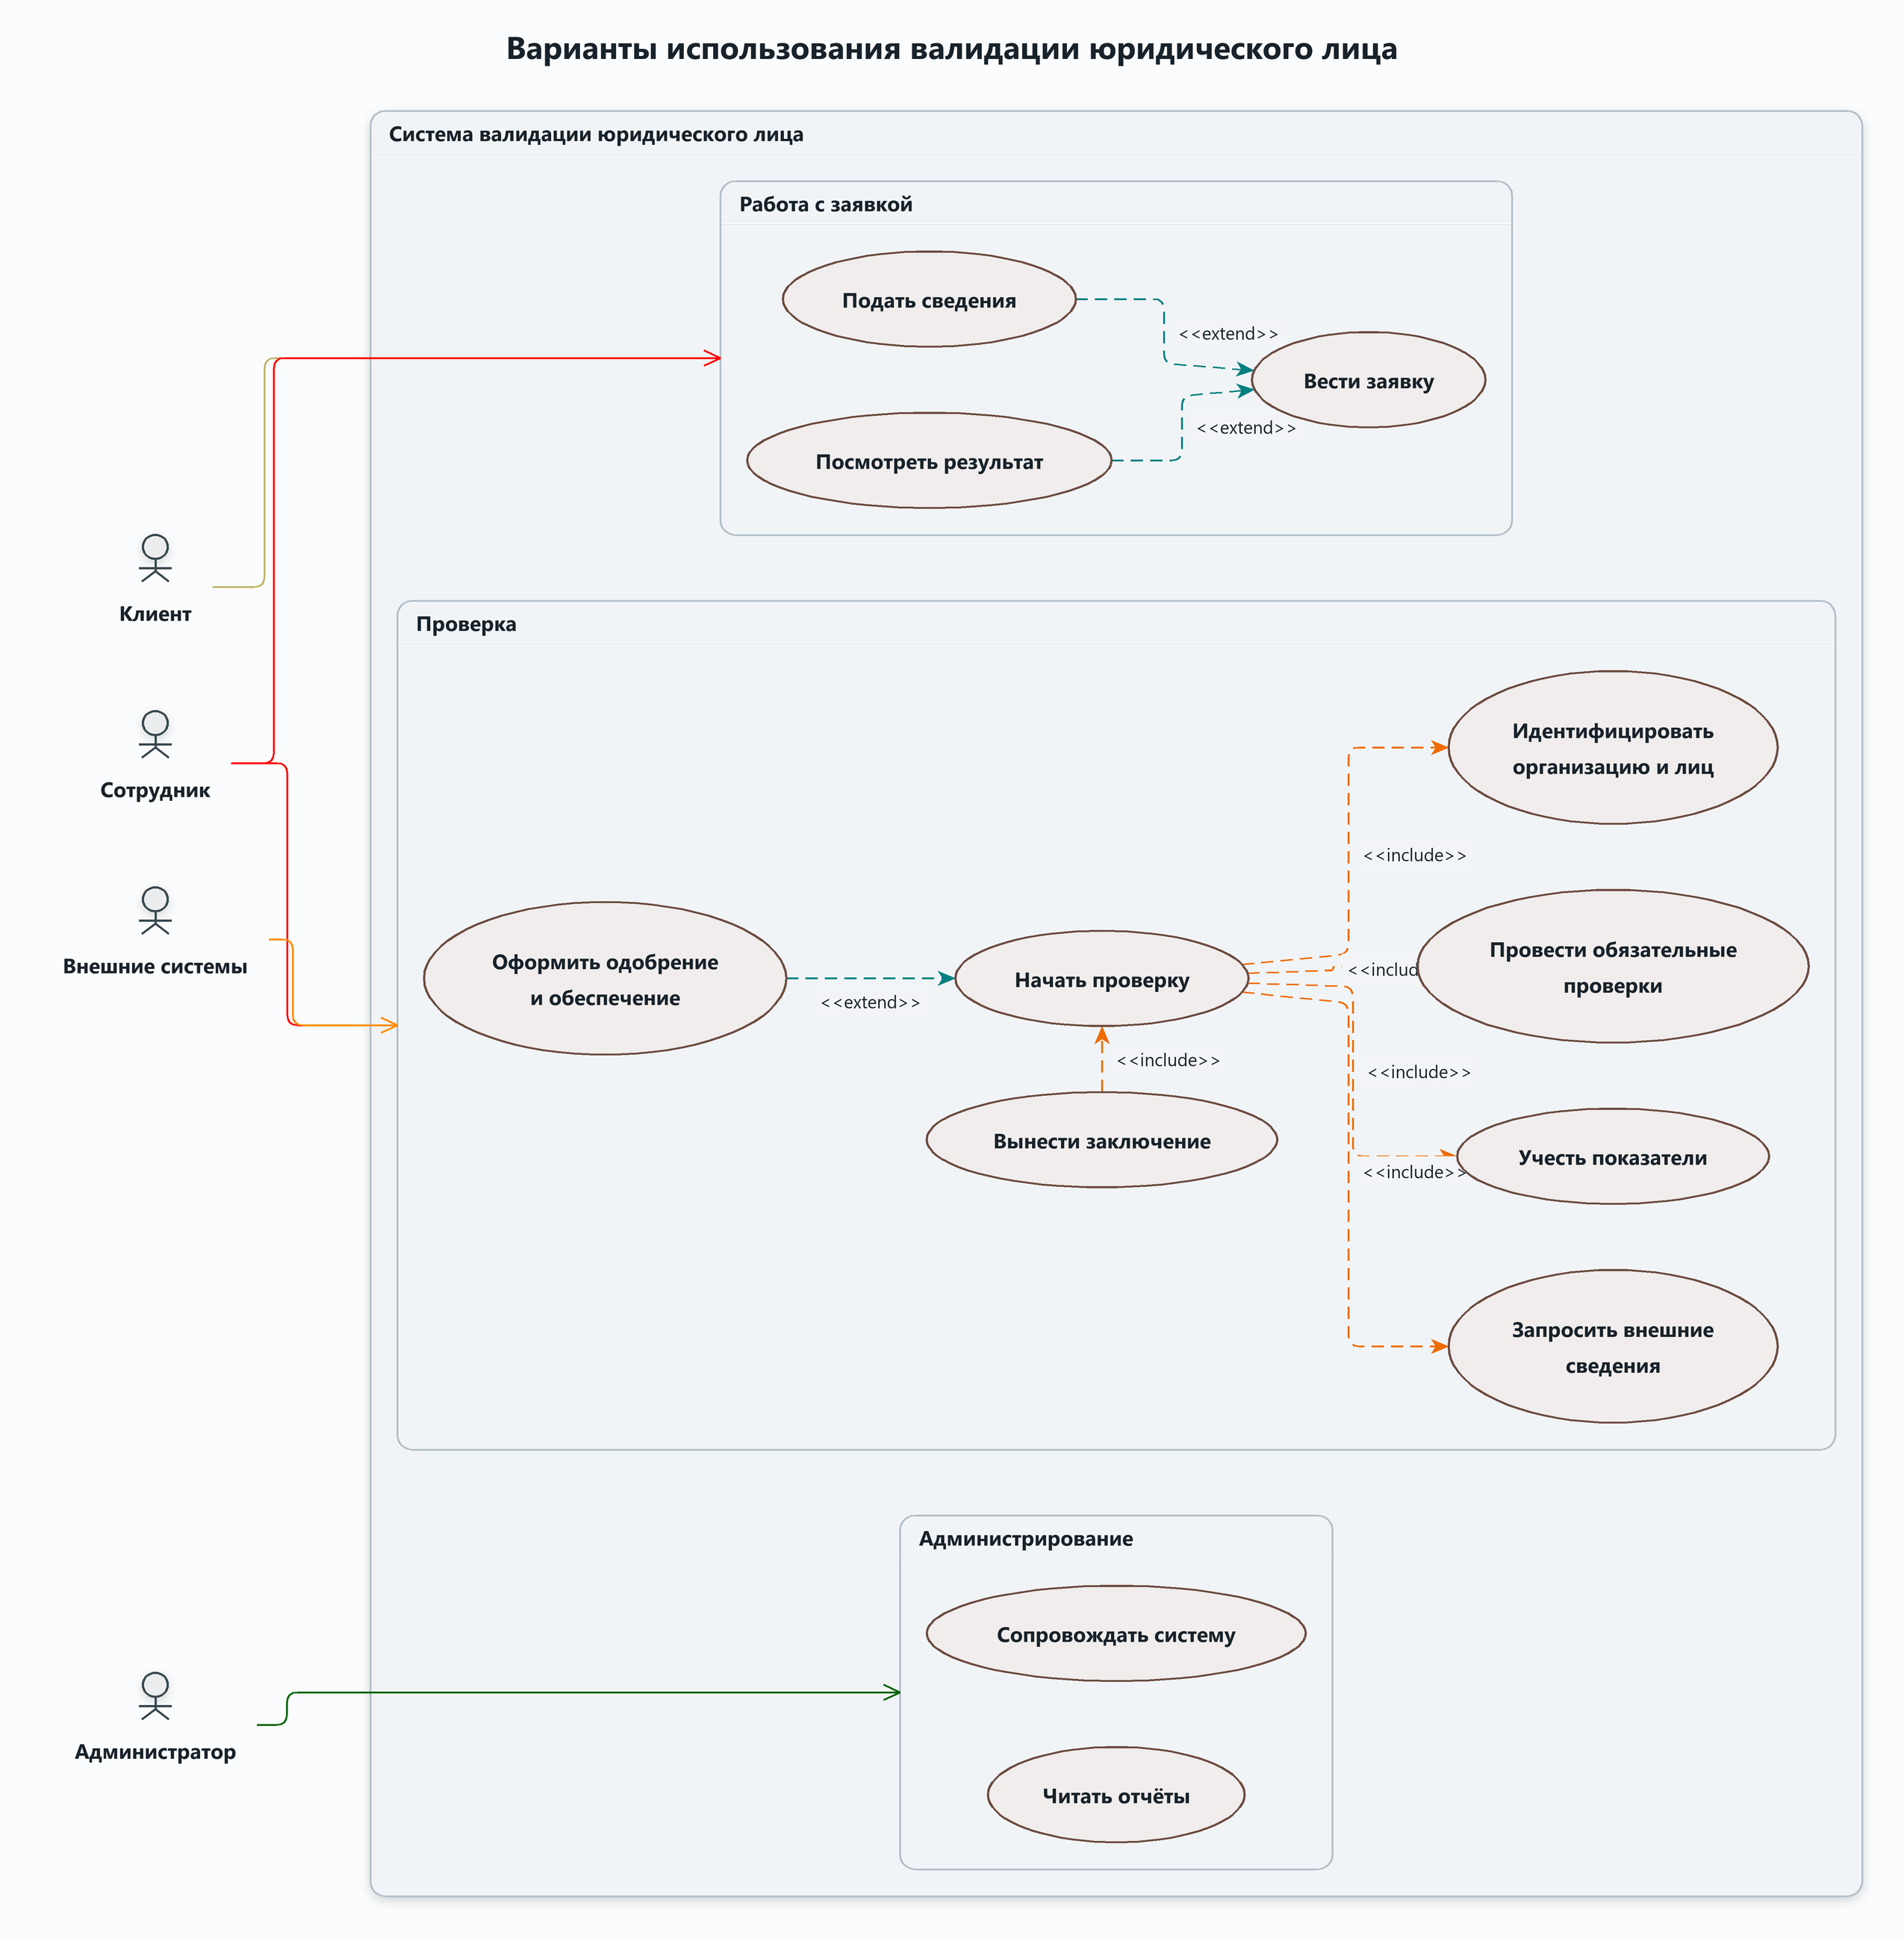
\includegraphics[width=\textwidth]{use_case_validaciya.png}
\caption{Диаграмма вариантов использования системы валидации юридического лица}
\label{fig:usecase}
\end{figure}

<<Подать сведения>> и <<Посмотреть результат>> расширяют вариант <<Вести заявку>>. <<Начать проверку>> включает идентификацию, обязательные проверки, учёт показателей и запрос внешних сведений. <<Оформить одобрение и обеспечение>> расширяет проверку: этих записей может не быть. <<Вынести заключение>> включает <<Начать проверку>>.

\subsubsection{Спецификация ключевых Вариантов Использования}

\textbf{Ведение заявки.}

Акторы: представитель юридического лица, клиентский менеджер.

Основной сценарий: представитель передаёт сведения об организации, лицах и долях. Менеджер создаёт заявку, указывает сумму, срок, валюту, канал и цель проверки и выбирает одни кредитные условия. Повторная проверка создаёт новую заявку.

Результат: заявка ссылается ровно на одни кредитные условия.

\textbf{Начало проверки.}

Акторы: клиентский менеджер, внешние системы.

Основной сценарий: менеджер отправляет заявку на проверку. Система идентифицирует организацию и участие, при длинной цепочке читает владение, проверяет действующее согласие и записывает обязательные проверки с нормой, источником и датой. Внешние сведения запрашиваются, когда проверка использует персональные данные или кредитную историю. Заявка на проверке без обязательной проверки не принимается.

Результат: у заявки есть одна или несколько обязательных проверок.

\textbf{Учёт показателей.}

Акторы: кредитный аналитик.

Основной сценарий: аналитик вносит финансовую отчётность и показатели. Показатель без отчёта допустим, если источник~--- суд, налог или бюро. В заявку показатель попадает связью <<Учтено>>: вес, порог и вывод. Вывод~--- усиливает, ослабляет или блокирует. Новая редакция условий не меняет уже записанный вес.

Результат: у заявки зафиксированы учтённые показатели с выводом по её условиям.

\textbf{Вынесение заключения.}

Акторы: андеррайтер.

Основной сценарий: андеррайтер читает проверки, учтённые показатели, условия, одобрение и обеспечение. Непройденная обязательная проверка или вывод <<блокирует>> закрывают положительный результат. Заключение получает результат, уровень риска, срок действия и, при отказе, причину. Пересмотр добавляет новое заключение и сохраняет предыдущее.

Результат: у заявки есть заключение. Офис и интернет-банк получают один уровень риска при тех же организации, показателях и условиях.

\textbf{Ведение цепочки владения.}

Акторы: специалист финансового мониторинга.

Основной сценарий: специалист записывает участие и владение: долю, основание, руководителя и бенефициара. Косвенная доля считается произведением долей по цепочке. Бенефициарный владелец~--- физическое лицо.

Результат: цепочка организаций и участия сохранены вместе с клиентом.

\textbf{Отчёты и сопровождение.}

Акторы: руководитель, администратор правил хранения, администратор системы.

Основной сценарий: руководитель читает отчёты по заявкам, отказам и уровню риска. Администратор правил задаёт категорию, основание, срок и событие начала отсчёта. Администратор системы заводит сотрудников и назначает роли.

Результат: правила хранения и роли заданы, отчёт сформирован.

\subsubsection{Дополнительные функциональные требования}

\begin{itemize}
\item поиск организации и заявки по ИНН, ОГРН, наименованию и номеру заявки;
\item запрос кредитной истории и иных внешних сведений только при действующем согласии;
\item выгрузка отчёта руководителя в PDF;
\item журнал действий сотрудников со сроком хранения пять лет;
\item неотправленный черновик заявки живёт один год и в пакет заявки не входит.
\end{itemize}

\subsection{Требования к экранным формам}

\begin{itemize}
\item \textbf{Форма входа.} Логин, пароль и роль. Дальше открываются только разделы этой роли.
\item \textbf{Главное меню.} Организация, заявки, проверки, отчёты, правила хранения. Состав пунктов зависит от роли.
\item \textbf{Карточка организации.} Наименование и организационно-правовая форма, ИНН, ОГРН и ОКВЭД, статус, адрес, лицензия, участия, владение и согласия.
\item \textbf{Форма заявки.} Номер, дата и канал, сумма, срок и валюта, статус и цель, выбранные кредитные условия, проверки, связь <<Учтено>>, одобрение, обеспечение и заключения.
\item \textbf{Форма заключения.} Результат проверки, уровень риска, срок действия и причина отказа. Представитель видит по своей заявке результат, срок и причину отказа.
\item \textbf{Форма отчётов и правил хранения.} Период, статус и уровень риска. Отдельно~--- категория сведений, основание, срок и событие начала отсчёта.
\end{itemize}

\subsection{Нефункциональные требования}

\textbf{Производительность.} Система обеспечивает одновременную работу сотрудников офиса и представителей в интернет-банке: не менее 200 сеансов. Время отклика при чтении карточки и заявки не превышает 2 секунд, при записи заявки, проверки и заключения~--- 3 секунд.

\textbf{Надёжность.} База защищает данные при сбое и восстанавливается из резервной копии до последнего согласованного состояния. Заявка, проверки, записи <<Учтено>> и заключение фиксируются одной транзакцией. Снятие пакета не удаляет клиента, показатель и редакцию условий.

\textbf{Безопасность.} Доступ разделён по ролям обзора. Представитель читает только свою заявку. Пароли хранятся в хешированном виде. Персональные данные и кредитная история обрабатываются при действующем согласии и по требованиям законодательства о персональных данных и о противодействии отмыванию доходов.

\textbf{Масштабируемость.} Новая редакция кредитных условий, новый вид обязательной проверки и новый канал подачи добавляются без смены уже накопленных заявок. Четыре категории хранения сохраняют свои сроки.

\section{Концептуально-информационная модель предметной области}

\subsection{ER-диаграмма модели}

\begin{figure}[p]
\centering
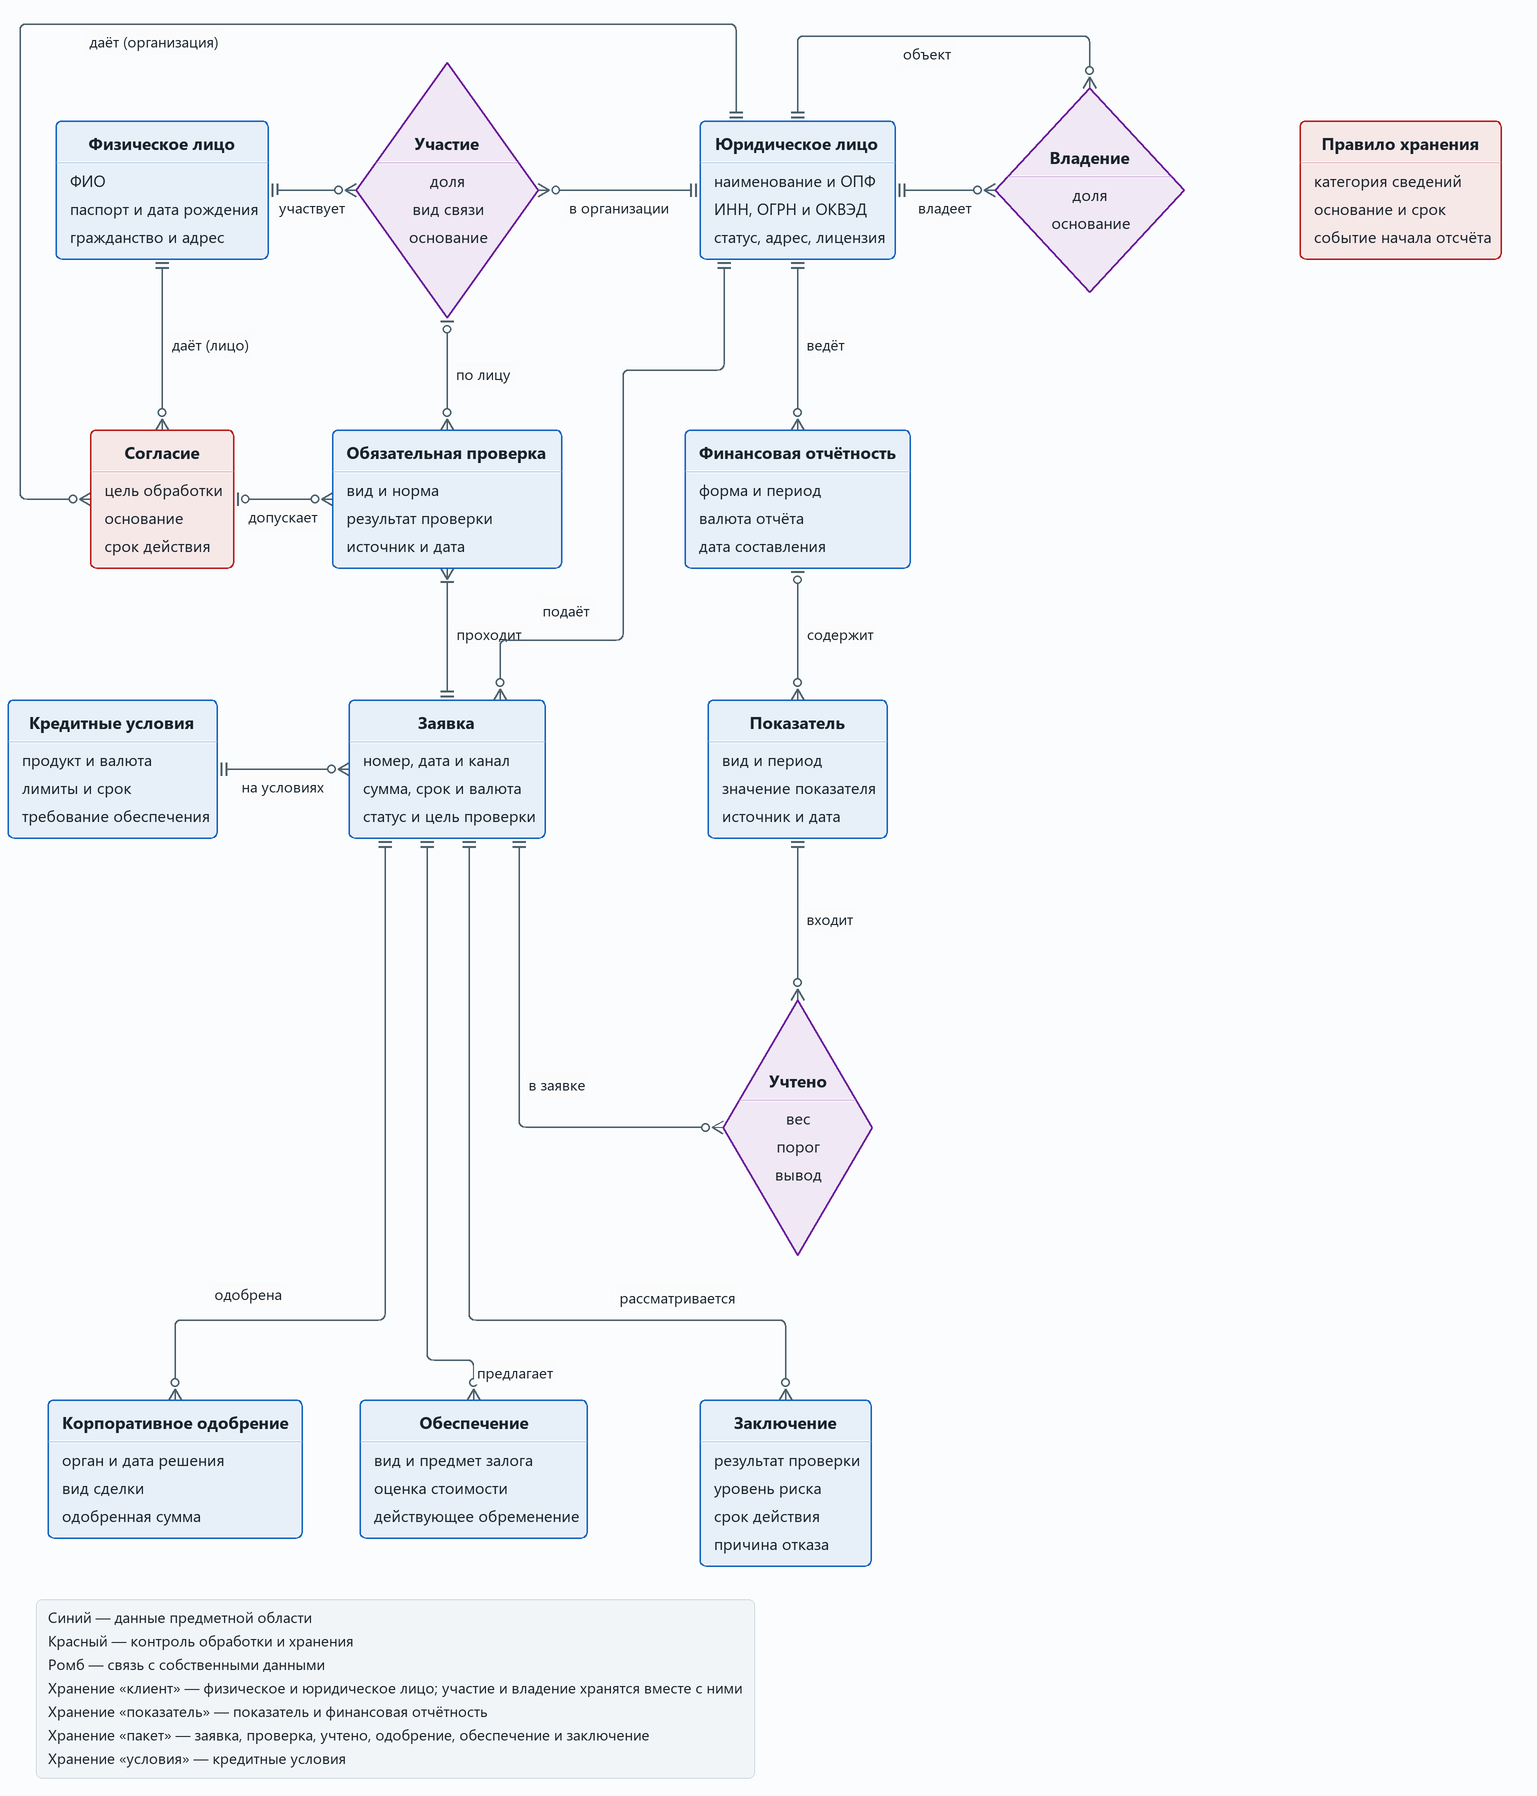
\includegraphics[width=\textwidth,height=0.88\textheight,keepaspectratio]{kmpo_validaciya_v9.png}
\end{figure}


\end{document}


